\documentclass[12pt,a4paper,oneside]{report}
\usepackage{indentfirst}
\usepackage{times}
\setlength\parindent{6ex}
\renewcommand{\baselinestretch}{1.50}\normalsize
\usepackage{anysize}
\marginsize{1.25in}{.75in}{1in}{1in}
\usepackage{graphics}
\usepackage{graphicx}
\usepackage{epsfig}
\usepackage[fleqn]{amsmath}
\usepackage{amsfonts}
\usepackage{textcomp}
\usepackage{graphicx}
\usepackage{float}
\usepackage{enumitem}
\usepackage{setspace}
\usepackage{fancyhdr}
\usepackage{truncate}
\usepackage{nomencl} 
\usepackage{acronym}
\usepackage{array}
\usepackage{caption}
\usepackage{cite}
\usepackage{subcaption}
\usepackage[overload]{textcase}
\usepackage{listings}
\renewcommand{\nomname}{List of Abbreviations}
\usepackage{makeidx}
\makeindex
\makenomenclature
\newcommand{\quotes}[1]{``#1''}
\usepackage{titlesec}
\titleformat{\chapter}[display]
{\normalfont\Large\bfseries\centering}
{\chaptertitlename\ \thechapter}{15pt}{\LARGE}
\titleformat{\section}{\large\bfseries}{\thesection}{1em}{}
\titleformat{\subsection}{\normalsize\bfseries}{\thesubsection}{1em}{}
\renewcommand{\chaptermark}[1]{\markboth{ \emph{#1}}{}}

\printnomenclature[5em]
\pagestyle{fancy}
%\headheight 1pt
	\renewcommand{\footrulewidth}{1.2pt}
\renewcommand{\headrulewidth}{1.2pt}
\rhead{\scriptsize {\leftmark}}

\lhead{\small{College of Engineering, Cherthala \;\;\;\;\;\;\;\;\;\;\;\;\;\;\;\;\;\;}}
\rfoot{\thepage}
\cfoot{\empty}
\lfoot{\small{Department of Computer Science \& Engineering}}
\renewcommand{\figurename}{Fig.}
\begin{document}
\renewcommand\bibname{References}
\begin{titlepage}
\begin{center}
\Large{\textbf{A SEMINAR REPORT ON}}\\
\vspace{.2 in}
\begin{singlespace}
\LARGE{\textbf{Leakage-Resilient Password Entry on Head-Mounted Smart Wearable Glass Devices }}\\
\end{singlespace}
\vspace{.2 in}
\Large{\textit{Submitted By }}\\
\Large{\textit{\textbf{ABHIJITH K D}}} \\
\textbf{Reg. No . CEC17CS002}\\
\Large{\textit{\textit{under the esteemed guidance of}}}\\
\Large{\textit{Mrs. Anitha M A}}\\
\Large{\textit{Assistant Professor}}\\
\Large{\textit{Computer Science \& Engineering}}
\vspace{.05in}
\begin{figure}[h]
\begin{center}
\epsfig{width=1.5 in, file=logo.jpg}
\end{center}
\end{figure}
\begin{singlespace}
\large{\textbf{OCTOBER 2020}}\\
\vspace{.2in}
\large{\textbf{DEPARTMENT OF COMPUTER SCIENCE AND ENGINEERING\\COLLEGE OF ENGINEERING,CHERTHALA\\ PALLIPPURAM P O, ALAPPUZHA-688541, \\PHONE: 0478 2553416, FAX: 0478 2552714\\http://www.cectl.ac.in}}
\end{singlespace}
\end{center}
\end{titlepage}

\begin{titlepage}
\begin{center}

\large{\textbf{A SEMINAR REPORT ON}}\\
\begin{singlespace}
\LARGE{\textbf{Leakage-Resilient Password Entry on Head-Mounted Smart Wearable Glass Devices}}\\
\end{singlespace}


\Large{\textit{Submitted By }}\\
\Large{\textit{\textbf{ABHIJITH K D}     (\textbf{Reg. No . CEC17CS002})}}\\
\Large{\textit{\textit{under the esteemed guidance of}}}\\
\Large{\textit{Mrs. Anitha M A}}\\
\begin{singlespace}
\large{\textit{In partial fulfillment of the requirements for the award of the degree}\\
\large{ \textit{of}}\\
\large{\textit{Bachelor of Technology} }\\
\large{\textit{in}}\\
\large{\textit{Computer Science and Engineering}}\\
\large{\textit{of}}\\
\large{\textit{APJ Abdul Kalam Technological University}}}\\
\end{singlespace}
\begin{figure}[h]
\begin{center}
\epsfig{width=1.5 in, file=logo.jpg}
\end{center}
\end{figure}
\begin{singlespace}

\Large{\textbf{OCTOBER 2020\\Department of Computer Science and Engineering\\College of Engineering, Pallippuram P O, Cherthala, Alappuzha Pin: 688541, \\Phone: 0478 2553416, Fax: 0478 2552714\\http://www.cectl.ac.in}}
\end{singlespace}
\end{center}
\end{titlepage}


\begin{titlepage}
\begin{center}

\large{\textbf{DEPARTMENT OF COMPUTER SCIENCE \& ENGINEERING}}\\
\large{\textbf{COLLEGE OF ENGINEERING CHERTHALA\\ALAPPUZHA-688541}}\\
\end{center}
\begin{figure}[h]
\begin{center}
\epsfig{width=1.5in, file=logo.jpg}
\end{center}
\end{figure}
\begin{center}
\large{\textbf{C E R T I F I C A T E}}\\
\end{center}
\begin{spacing}{1.5}
This is to certify that, the seminar report titled  \textbf{\textit{ Leakage-Resilient Password Entry on Head-Mounted Smart Wearable Glass Devices}} is a bonafide record of the \textbf{the CS451 SEMINAR AND PROJECT PRILIMINARY} presented by \textbf{ABHIJITH K D} (Reg.No.CEC17CS002), Seventh Semester B. Tech. Computer Science \& Engineering  student,  under our guidance and supervision, in partial fulfillment of the requirements for the award of the degree, \textbf{B. Tech. Computer Science  \& Engineering } of \textbf{APJ Abdul Kalam Technological University.}.
\end{spacing}
\begin{tabbing}
xxxxxxxxxxxxxxxxxxxxxxxxxxxxxxxxxxxxxx\= xxxxxxxxxxxxxxxxxxxx\= \kill
\hspace{.15in}{\bf Guide} \>\hspace{-.7in}{\bf Co-ordinator}\hspace{1.32in}{\bf  HoD  } \\
\end{tabbing}
\begin{tabbing}
xxxxxxxxxxxxxxxxxxxxxxxxxxxxxxxxxxxxxx\= xxxxxxxxxxxxxxxxxx\= \kill
%\vspace{0.3in}\\
\hspace{.15in}{\bf{Mrs. Anitha M A}}   \>\hspace{-.7in}{\bf Mrs. Janu R Panicker} \hspace{.65 in}{\bf Dr. Priya S}\\
\hspace{.15in}Assistant Professor    \>\hspace{-.7in}Assistant Professor\>\hspace{.05in} Professor\\
\hspace{.1in} Computer Science \& Engg.    \>\hspace{-.75in}    Computer Science \& Engg. \>\hspace{.035in}    Computer Science \& Engg.\\

\end{tabbing}
\end{titlepage}


\renewcommand*\thesection{\thechapter.\arabic{section}}
%\pagenumbering{arabic}
%\addtocounter{page}{4}

\begin{titlepage}
\pagenumbering{roman}
%\addtocounter{page}{4}
\setcounter{page}{4}
\section*{\begin{center} \Large{ACKNOWLEDGEMENT }\end{center}}

\thispagestyle{plain}


%{$\;\;\;\:$}
\par
This work would not have been possible without the support of many people.
First and the foremost, I give thanks to Almighty God who gave me the inner strength, resource and ability to complete my seminar successfully.
\par
I would like to thank \textbf{Dr. Mini M G}, The Principal, who has provided with the best facilities and atmosphere for the seminar completion and presentation. I would also like to thank HoD \textbf{Dr. Priya S} (Professor, Computer Science and Engineering) and my seminar guide \textbf{Mrs. Anitha M A} (Assistant Professor, Computer Science and Engineering), my seminar coordinator \textbf{Mrs. Janu R Panicker} (Assistant Professor, Computer Science and Engineering) for the help extended and also for the encouragement and support given to me while doing the seminar.
\par
I would like to thank my dear friends for extending their cooperation and encouragement throughout the seminar work, without which I would never have completed the seminar this well. Thank you all for your love and also for being very understanding. 

\end{titlepage}
\newpage

\section*{\begin{center}\Large ABSTRACT\end{center}}
\thispagestyle{plain}
\setcounter{page}{5}
\par
\hspace{0.1in}
With the boom of Augmented Reality (AR) and Virtual Reality (VR) applications, head-mounted smart wearable glass devices are becoming popular to help users access various services like E-mail freely. However, most existing password entry schemes on smart glasses rely on additional computers or mobile devices connected to smart glasses, which require users to switch between different systems and devices. This may greatly lower the practicability and usability of smart glasses. Moreover the existing systems password entry schemes are not that much secure and there is a high chance of Eavesdropping attacks.
\par This paper focus on these challenges and design three practical anti-eavesdropping password entry schemes on stand-alone smart glasses, named gTapper, gRotator and gTalker. The main idea is to break the correlation between the underlying password and the interaction observable to adversaries. Based on the analysis of an IRB-approved user study, these schemes are found to be easy-to-use without additional hardware under various test conditions, where the participants can enter their passwords within moderate time, at high accuracy, and in various situations.
\\
\\\hspace{-.43in} 
\textbf{Keywords--} \textit{\textbf{Smart glasses, Leakage-Resilient Password Entry, Augmented Reality - Virtual Reality }}

%\pagenumbering{arabic}
%\setcounter{page}{5}
\tableofcontents
%\pagenumbering{arabic}
%\listoftables
\listoffigures
%\listoftables



%\renewcommand*\thesection{\thechapter.\arabic{section}}
\newpage
\pagestyle{fancy}
\headheight 26pt
\renewcommand{\footrulewidth}{1.2pt}
\renewcommand{\headrulewidth}{1.2pt}
\rhead{\scriptsize {\leftmark}}
%\chead{Middle top}
\lhead{\small{College of Engineering, Cherthala \;\;\;\;\;\;\;\;\;\;\;\;\;\;\;\;\;\;}}
\rfoot{\thepage}
\cfoot{\empty}
\lfoot{\small{Department of Computer Science \& Engineering}}
\pagenumbering{arabic}
\chapter{INTRODUCTION}
\label{intro}
%\pagenumbering{arabic}
%\setcounter{page}{1}
%\hspace{0.1in}

\par
Due to the convenient and efficient capability of connecting individuals and cyberspace, head-mounted smart
wearable devices[13] are becoming prevalent, e.g., smart glasses.
By wearing compact and lightweight smart glasses, users can
access various services, such as personal email and online
social network, and map services, in a hand-free manner at
any place and at any time, through Augmented Reality (AR)
or Virtual Reality (VR) [2], [3]. To protect these devices from
unauthorized access, password-based user authentication has
been pervasively used to validate users’ identity. However,
such authentication mechanism has intrinsic vulnerabilities,
e.g., eavesdropping attackers can leak users’ password by
directly or indirectly observing password entry procedure via
accessible channels. This kind of attack is particularly effective
in practical scenarios, since smart glasses are usually used
in public areas and outdoors that are vulnerable to password
leakage.
\par
In order to thwart the threat of eavesdropping attacks, prior
research focuses on improving anti-eavesdropping password 
entry on desktops, laptops, smartphones and tablets [5].
However, most of them suffered from both security and usability issues. To achieve better security and
usability, it is necessary to use a protected environment to
hide certain user interaction during the password entry [6]. While this solution is not suitable to protect password
entry on smart glasses due to the following reasons. Firstly,
the traditional input equipment like keyboard and touch screen
is not available on the smart glasses according to the compact
and lightweight design. Secondly, smart glasses have a much
smaller screen than the PC monitors and phone screens. Then,
smart glasses have limited hardware support.
\par



\begin{figure}[H]
    \begin{center}
        \label{abc}
            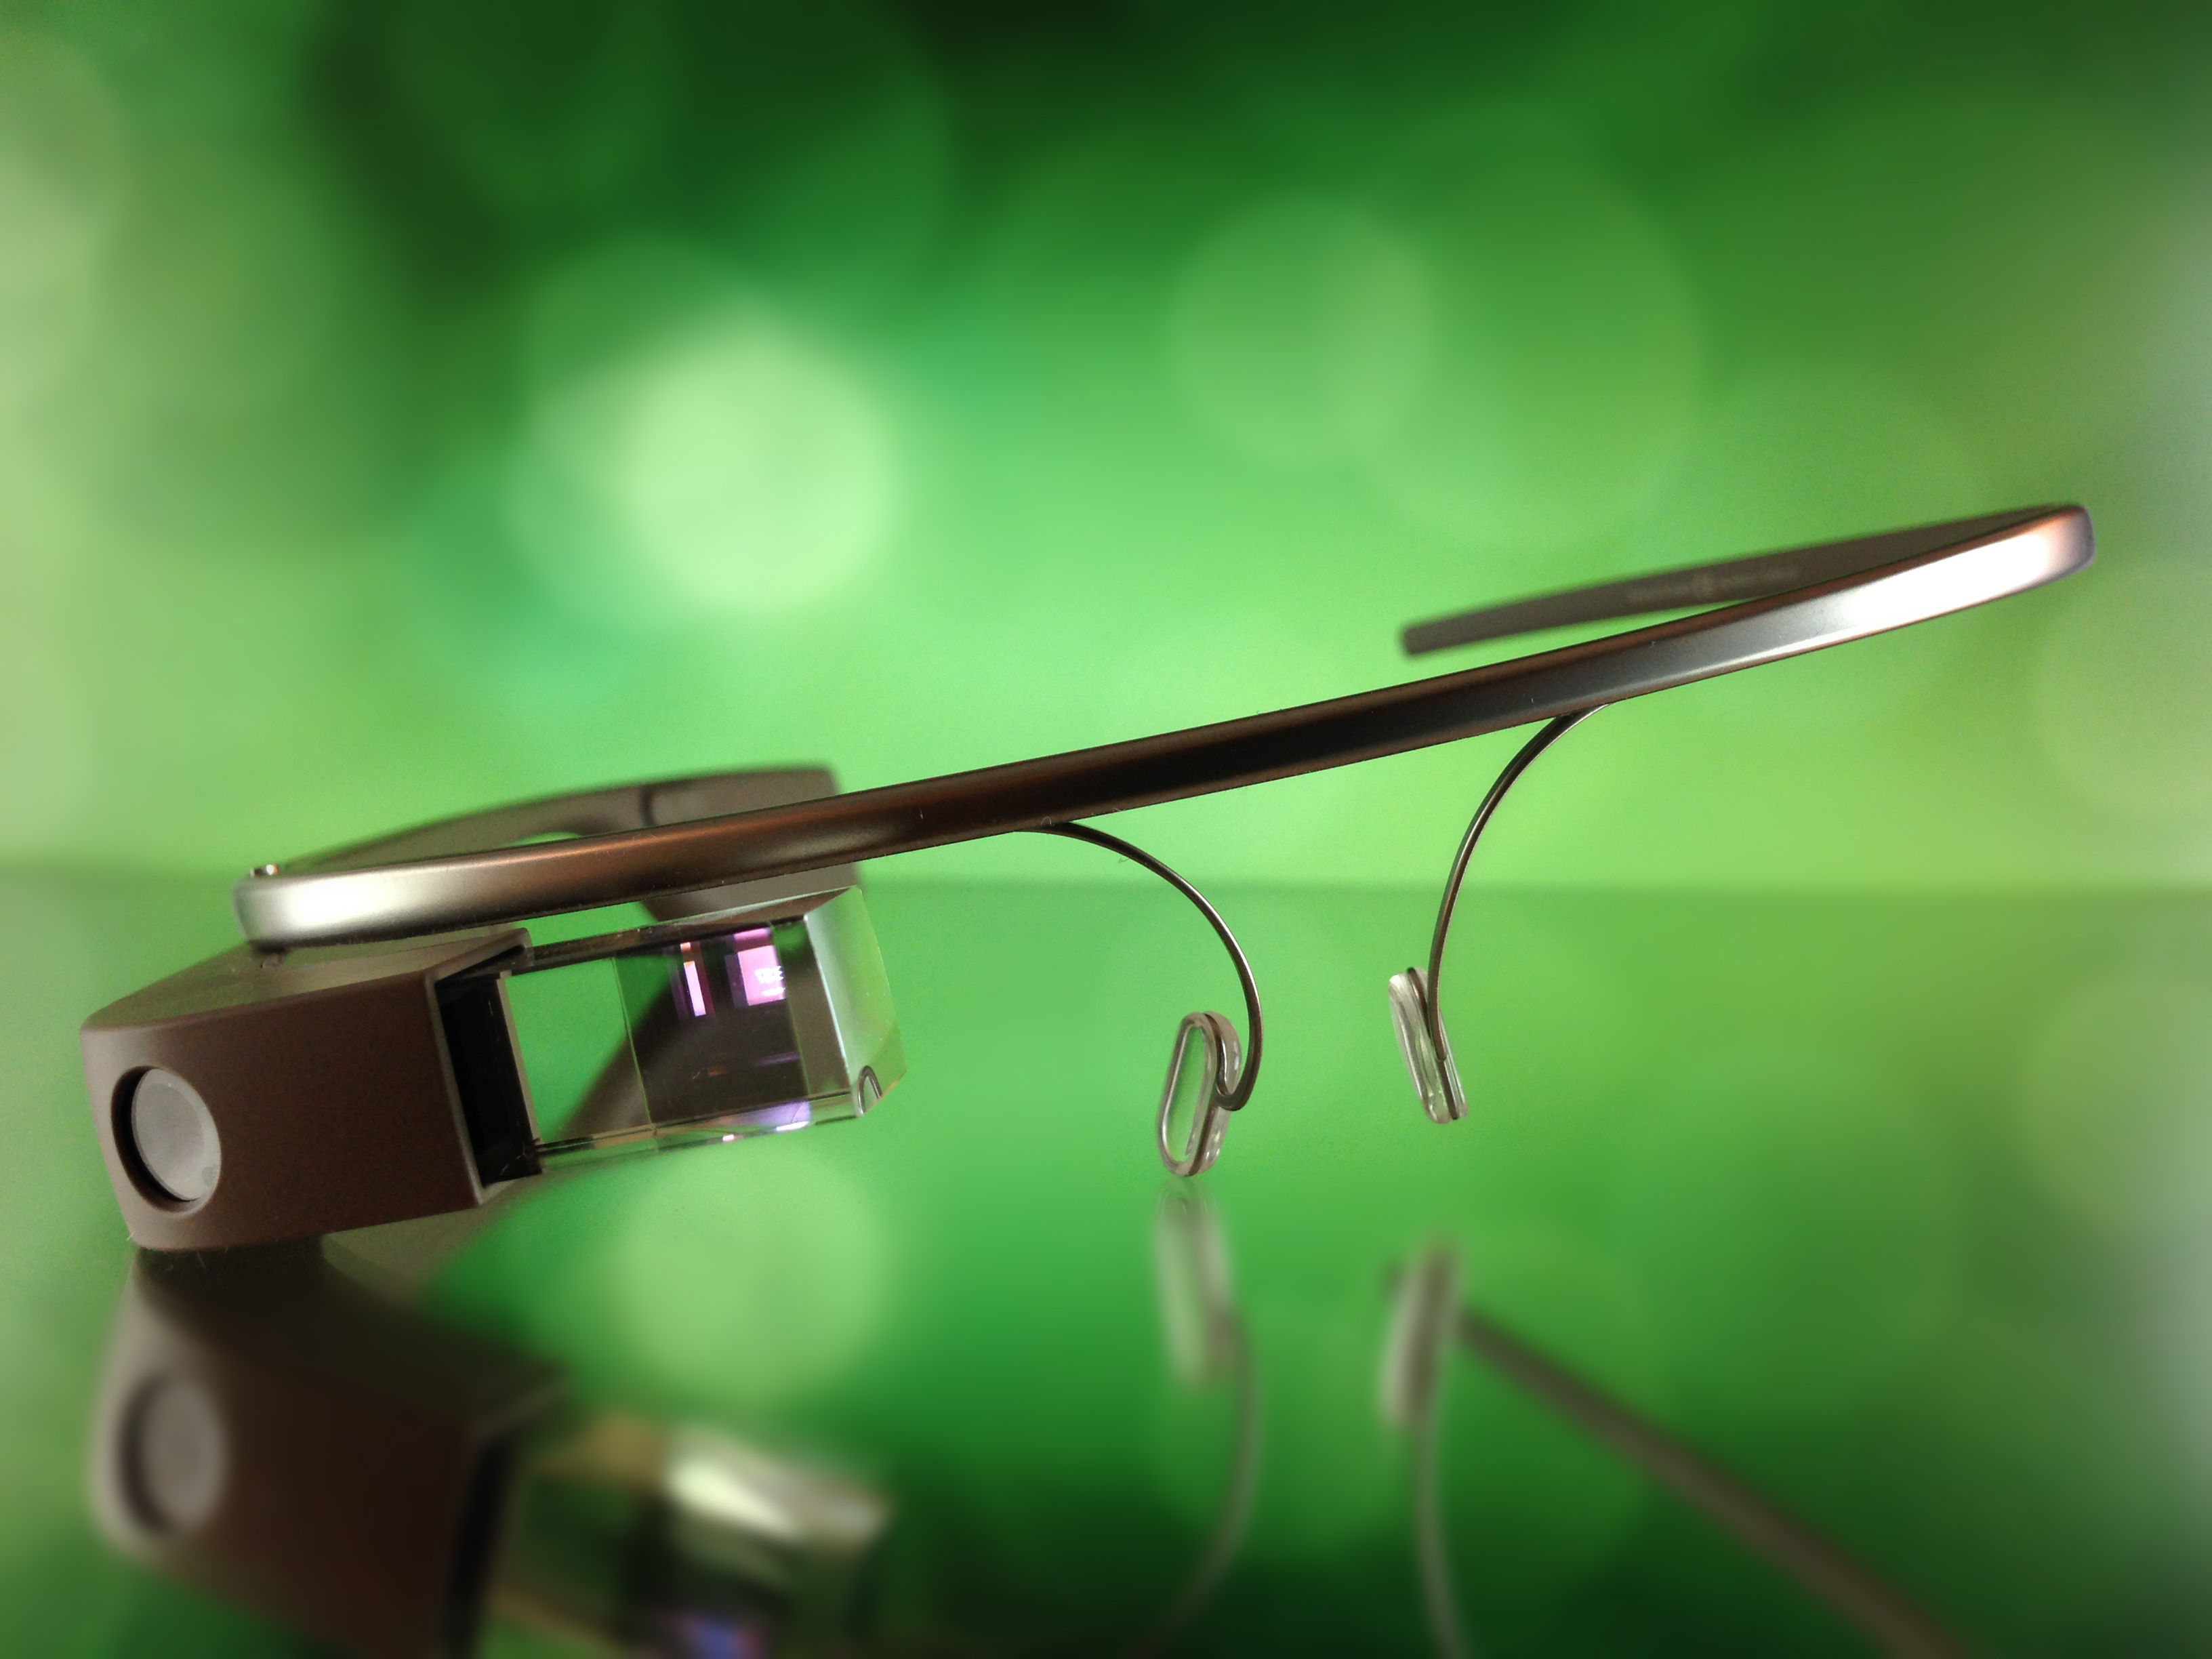
\includegraphics[scale=.1]{Google_Glass.jpg}
            \caption{Google Glass[3]}
    \end{center}
\end{figure}
\begin{figure}[H]
    \begin{center}
        \label{abc}
            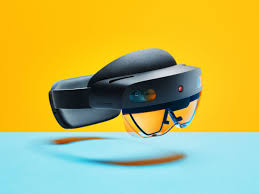
\includegraphics[scale=1.3]{hlololensjpg.jpg}
            \caption{HoloLens by Microsoft[4]}
    \end{center}
\end{figure}

\newpage
This paper focus on Google Glasses as it is more popular than HoloLens in the current scenario on market.\newline
\textbf{ Google Glass,} or simply Glass, is a brand of smart glasses—an optical head-mounted display designed in the shape of a pair of eyeglasses. It was developed by X (previously Google X) with the mission of producing a ubiquitous computer. Google Glass displays information in a smartphone-like, hands-free format. Wearers communicate with the Internet via natural language voice commands. \begin{figure}[H]
    \begin{center}
        \label{abc}
            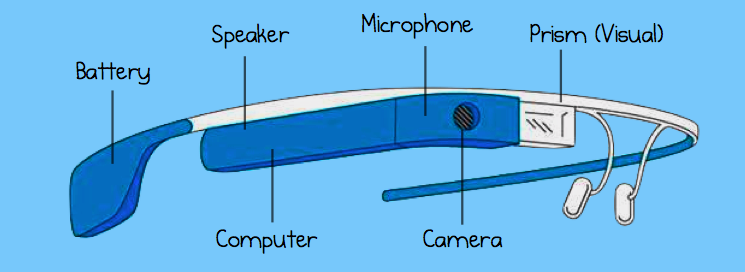
\includegraphics[scale=.4]{components.png}
            \caption{Parts of Google Glass}
    \end{center}
\end{figure}
\begin{itemize}
\item \textbf{Touchpad:} A touchpad is located on the side of Google Glass, allowing users to control the device by swiping through a timeline-like interface displayed on the screen. Sliding backward shows current events, such as weather, and sliding forward shows past events, such as phone calls, photos, circle updates, etc.
\item \textbf{Camera:} Google Glass has the ability to take 5 MP photos and record 720p HD video. Glass Enterprise Edition 2 has an improved 8MP 80° FOV[8] camera.
\item \textbf{Display:} There is a display called Near-Eye-Display available in the google glass. It's actually a prism which have display properties. As it is very near to the wearer's eye, the possibility of data observation which is displayed in the screen is not possible.
\item \textbf{Microphone:} A microphone is availabale in the Google glass which is used to receive the audio input from the user and to process it.
\end{itemize}
\chapter{EXISTING SYSTEM}

\section{Existing Password Entry Schemes}

There exist many user authentication schemes (password entry schemes)  have been proposed to resist against eavesdropping attacks. Some of the major password entry schemes that are popularly used are discussed in this section.
 \par 
 Ginzburg et al. [9] proposed an authentication scheme that
can verify users via random challenges, but the scheme
workload is high as users have to memorize a formula for
authentication.
  Weinshal [10] designed a CAS scheme based
on the cognitive capability of human beings. It requires a
user to identify around 30 secret pictures and find out a
path among 80 pictures randomly displayed on the screen
in only one single round. According to the analysis in [10],
CAS may expose a high usability cost, which may take
up to 221 seconds per login attempt. Moreover, it requires
10 rounds of authentication attempts to mitigate brute-force
attacks. Then, some eye-gaze based schemes were proposed
for inputting passwords [29]. Unfortunately, such schemes
require extra hardware-based eye-tracking tools that are often
not available on existing smart glasses.

\par Li et al. [11] proposed a scheme, called CoverPad, to protect
the password entry process on mobile phones and tablets
with acceptable usability. It leverages a temporary secure
channel between user and touch screen in order to transform
a password during the password entry. This aims to prevent
an adversary from inferring any information by monitoring
a user’s inputting behaviour. Due to the compact and lightweight design of smart glasses, it is difficult to apply the
existing anti-eavesdropping password entry schemes to smart
glasses.

\par Li et al. [1] designed a series of anti-eavesdropping
password entry schemes for smart glasses and presented
preliminary results of the scheme performance. This work
significantly extends the above work in four major aspects.
Firstly, an important internal eavesdropping adversary model
is introduced and analyzed. Secondly, the experiments involve
distraction levels, multiple modalities, and six test cases that
are important to evaluate the usability and practicability of the
schemes in real-world scenarios. Thirdly, more comprehensive
and thorough evaluation and analysis are provided. Fourthly,
a more thorough literature review is presented.

\section{Eavesdropping Attack}

An eavesdropping attack[12], also known as a sniffing or snooping attack, is a theft of information as it is transmitted over a network by a computer, smartphone, or another connected device.
The attack takes advantage of unsecured network communications to access data as it is being sent or received by its user.
Eavesdropping is a deceptively mild term. The attackers are usually after sensitive financial and business information that can be sold for criminal purposes. There also is a booming trade in so-called spouseware, which allows people to eavesdrop on their loved ones by tracking their smartphone use.
An eavesdropping attack can be difficult to detect because the network transmissions will appear to be operating normally.\newline This type of attacks against password entry can be categorized into 
\begin{itemize}
    \item External eavesdropping
    \item Internal eavesdropping
\end{itemize}
 Depending on the exploitable
attack channels, the former can be further classified into
\begin{itemize}
    \item Vision-based attack
    \item Motion-based attack
    \item Acoustics-based attack
\end{itemize}
 Under the vision-based attack, an adversary can
directly view or record videos about a victim’s password entry
and then infer the victim’s password by analyzing various
clues in the video. 2) Under the motion-based attack,
an adversary may attack remotely by accessing arm-mounted
motion sensors equipped on a smart wearable device[13]. For instance, Liu et al. explored such threat by
showing the feasibility of inferring users’ PINs and typed texts
through sensor data on smart watch. Wang et al. further
demonstrated that motion data from wrist-worn devices can be
used to distinguish mm-level distances in users’ hand movements during password input. 3) Under the acoustics-based
attack, an adversary can record audio signals about password
entry and infer a victim’s password by analyzing the ringtones
and keystroke acoustics from the recorded audio [20].

\par 
On the other hand, internal eavesdropping attacks can
be further classified into unprivileged attacks and privileged
attacks. The first type of attacks can be launched by an
adversary based on unprivileged access to password entry data.
As a typical example, as the motion sensor data on smart
devices could be accessed by any applications, an adversary
may recover a victim’s movements during the password entry
process and then find the underlying password. By contrast, the second type of attacks allows an adversary to reach
the internal memory of a victim’s device via malware, logic
key logger, and network traffic monitor [14]. It is worth noting
that the proposed designed schemes can be used to mitigate the unprivileged attacks, while may still be subject to the privileged
attacks that can be controlled by other security mechanisms
and proper configuration of operating systems.




\section{Problem Definition}

Most existing password entry schemes on
smart glasses require users to input their passwords by connecting the glasses with additional PCs or mobile devices,
whereas the additional devices may not be always available or accessible in certain scenarios, especially in public
places and outdoors. In this case, users may need to switch
between smart glasses and mobile devices for password entry.
Such interrupted user experience may lead to more inputting
errors, and even raise users’ stress and anxiety [10] when
they perform important tasks like AR-based or VR-based
payment [15]. Moreover, Near-Eye-Display (NED) screens
have also been exploited on Google Glass, which is a tiny
optical instrument to reflect and magnify the display to users’
eyes. It is found that the NED screen can help solve
part of password leakage, but is still hard to fully protect the
password entry. As a result, how to design a secure and
usable anti-eavesdropping password entry scheme for smart
glasses remains a challenge.



\par
This paper focus on this challenge
and design three anti-eavesdropping password entry schemes
for smart glasses, named gTapper, gRotator and gTalker.
As the NED screen has been widely deployed in smart glasses,
it plays an important role in proposed scheme design. There are
several features of a typical NED screen. 1) In order to
present clear and sharp display to users, the NED screen
is head-mounted. It is fixed on the smart glass frame and
placed physically close to the users’ eyes [3]. 2) Thanks to
its compact size and physical proximity to the users’ eyes,
the NED screen can privately display information to users
without being observed by others. This characteristic can be
used to deliver hidden information, breaking the correlation
between the underlying password and the interaction observable to an adversary.

\par
Due to these features, the  schemes that are going to propose do not require any
additional hardware or external devices other than a touch
pad, a gyroscope, and a microphone, which are commonly
available on smart glasses. To enter password, these schemes
require users to perform simple gestures on the touch pad,
slightly rotate head, or speak numbers based on the hidden
information displayed on the NED screen of smart glasses.
In the evaluation, design of the proposed schemes on
Google Glass, which is a popular commercial smart glasses,
and analysed the user study done by the authors of the base paper.


\chapter{PROPOSED SYSTEM}

\section{Design Overview}

\par
The proposed system introduces 3 new password entry schemes.  The main idea is to break the correlation between the underlying password and
the interaction observable to adversaries.
In existing password entry schemes on
smart glasses require users to input their passwords by connecting the glasses with additional PCs or mobile devices,
whereas the additional devices may not be always available or accessible in certain scenarios, especially in public
places and outdoors. In this case, users may need to switch
between smart glasses[13] and mobile devices for password entry.
\par
This section  introduce the design goals and three
anti-eavesdropping password entry schemes:
\begin{enumerate}
    \item gTapper
    \item gRotator
    \item gTalker
\end{enumerate} \newline
The architecture diagram of the google glass is given in the figure 3.1 . The above mentioned schemes only uses these hardware so that no extra hardware required for the proposed password entry schemes. The schemes gTapper, gRotator, gTalker uses the hardwares Touch Pad, Gyroscope[16] and Microphone respectively.

\begin{figure}[H]
    \begin{center}
        \label{abc}
            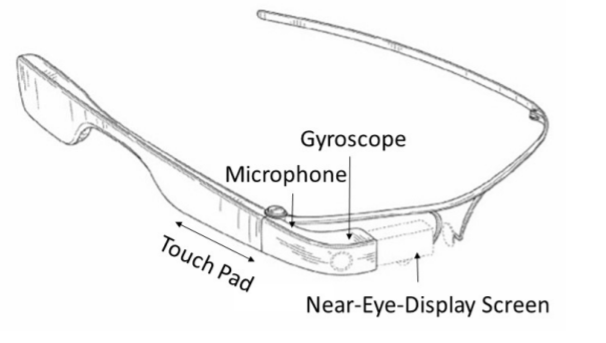
\includegraphics[scale=1]{google.png}
            \caption{Hardware of Google Glass that required for proposed scheme}
    \end{center}
\end{figure}
\par
Most existing smart glasses have typical built-in hardware
and sensors, including an NED screen, a touch pad, a gyroscope, and a microphone. Because of the tiny size and physical proximity to a user’s eye,
it is difficult for an adversary, even a hidden camera, to access
the channel between the NED screen and the users without
causing awareness. Thus, the designed schemes can use the
NED screen to display information privately to a user without
being noticed. In addition, designed schemes adopt a set of simple
and typical interaction operations on smart glasses, including
finger gestures, head movements and human voice by means
of the touch pad, gyroscope, and microphone. Overall, the scheme take
advantage of these hardware and interaction channels to design
the schemes on smart glasses. 
\par 
Regarding the proposed design, assume a server and a user agree
on a n-length password \newline pwd = ( $p_1$, $p_2$,..., $p_n$). For each
i $\epsilon$ \{0, 1, 2,..., 9\} in an authentication process, a hidden random
keypad $\Gamma_i$(·) is privately displayed to the user through the
NED screen on smart glasses during the process of password
entry. The hidden random keypad $\Gamma_i$(·) defines a random
mapping \newline $\Omega$ → $\Phi$ where $\Omega$ is the set of all elements contained
in the password alphabet and $\Phi$ is the set of all candidate
user operations via a user-device interaction channel. Note
that in each round i, a new random mapping $\Gamma_i$(·) (i.e., a new
hidden keypad) is drawn from the universal set of the candidate
mappings $\Omega$ → $\Phi$ following uniform distribution. Thus, given
the hidden keypad $\Gamma_i$(·), users have to perform corresponding
operations $op_i$ = $\Gamma_i$($p_i$) via the interaction channel in order
to select the correct underlying password element $p_i$ in pwd.

\par 
The observable response operation $op_i$ by the user for the
same password element is uniformly randomized due to the
hidden random keypad $\Gamma_i$(·). Therefore, as long as $\Gamma_i$(·) is not
disclosed, an adversary cannot infer any useful information
from $op_i$ to discover the underlying password element $p_i$,
even through external eavesdropping and unprivileged internal
eavesdropping attacks. As the hidden keypad is privately
delivered to the user via the NED screen, it is difficult for
adversaries to compromise this delivery channel. The detailed
security analysis will be discussed later in this section.
During the password entry process, different users may have
various response operations and hidden random mappings.


\section{Design Goals}

To design practical anti-eavesdropping of password entry
on smart glasses, it is important that the schemes do not need
to rely on any additional devices, which may not be always
available in a real environment. Even if these devices are
available, they may not resist against eavesdropping attacks.
In addition to retaining most benefits of traditional passwords,
our design goals can be explained from security, practicability,
and usability perspectives.
\begin{itemize}
    \item In order to protect password-based user authentication on
smart glasses, a desirable scheme should minimize the
threat of password leakage during the whole password
entry process. In practice, smart glasses can be often
used in various environments, especially public areas,
an adversary has a big opportunity to steal passwords,
including external eavesdropping and unprivileged internal eavesdropping as described in chapter 2. The
adversary can infer the credentials by observing the
entry process and analyzing the correlation between the
observed information and underlying password. As a
result, it is important to decouple the link in-between.
\item Then, a desirable scheme should be pervasively accessible
on smart glasses in practical settings. For this purpose,
it is preferable no additional devices or external to be
involved, as these devices or hardware may not be always
available or accessible in a real scenario like outdoor and
public areas. The scheme is expected to be constructed
by using the built-in hardware and functionalities, which
are commonly available on existing commodity smart
glasses.
\item A desirable scheme should provide good usability, i.e,
preserving the benefits of legacy password such as
nothing-to-carry and easy-to-use features. Therefore,
intuitive and simple operations are preferable for users
during the password entry, especially in inconvenient
environments, e.g., crowded places.
\end{itemize}


\section{gTapper}
\subsection{Design of gTapper}

This scheme of gTapper is designed based on the small
touch-pad that is widely available on most smart glasses [13].
The pad accepts users’ finger gestures as input signals,
including tapping, pressing, and swiping with different fingers
towards various directions.
\par 
Typically, this scheme adopts the password alphabet $\Omega$
to be comprised of all single-digit numbers from 0 to 9.
To implement gTapper, the hidden keypad contains 10 numbers
as shown in Figure 3.2. In each round i, gTapper randomly
selects a number $s_i$ $\epsilon$ \{0, 1, 2,..., 9\} and sets the focus
on that number $s_i$ , i.e., Figure 3.2 shows that the number
of 5 is focused in the hidden keypad.
\begin{figure}[H]
    \begin{center}
        \label{abc}
            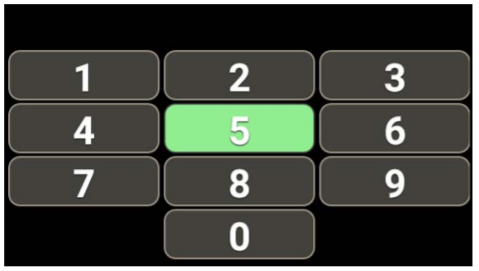
\includegraphics[scale=1]{gTapper.png}
            \caption{ Demonstration of gTapper}
    \end{center}
\end{figure}
\begin{figure}[H]
    \begin{center}
        \label{abc}
            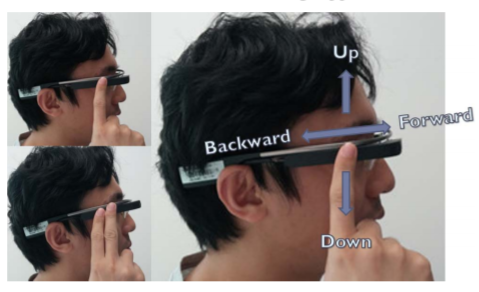
\includegraphics[scale=1]{touchpad.png}
            \caption{ Touch Gestures }
    \end{center}
\end{figure}

\par  It is worth noting
that users can locate the keys easily and swiftly, as the key
locations would not change. To change the number focus
in either descending or ascending order, users have to use
one finger to swipe forward or backward on the touch pad,
as shown in Figure 3.2. To summarize, users can use one
finger to shift the number focus to ($s_i$ − 1) mod 10 or
($s_i$ + 1) mod 10, by swiping forward once or by swiping
backward once. This scheme only consider two intuitive
gestures to shift focus like swiping forward/backward in order
to reduce users’ mental preparation and workload [33], which
is also examined and observed in the pilot study.
\par 
To enter a password element $p_i$ $\epsilon$ \{0, 1, 2,..., 9\} in round
i, a user has to shift the number focus to pi on the keypad
from the initially focused number $s_i$ by swiping forward or
backward for $op_i$ times, where opi = ($s_i$ − $p_i$) mod 10 or
$op_i$ = ($p_i$ − $s_i$si) mod 10 respectively. Then the user can enter
the selected number $p_i$ with a one-finger tap on the touch
pad. Taking Figure 3.2 as an example, if given an underlying
password element 7 and a hidden keypad in which the focused
number is set to 5, a user can select and enter this password
element 7 on the hidden keypad, by swiping backward with
one finger on the touch-pad for 2 = 7 − 5 times.\newpage


\subsection{Security Analysis of gTapper}

During the user’s password
entry, as attackers can directly or indirectly observe the user’s
operations in each round i through external eavesdropping
attacks and unprivileged internal eavesdropping attacks, they
can know user operations on gTapper including swiping forward/backward on the touch pad and the number of swiping
operations. Based on the observation in round i, attackers can
know the number and the directions of shifts from the initially
focused number to the i-th element of the password. However,
since the hidden keypad is protected, it is hard for attackers
to know what the initially focused number is and therefore
cannot infer the i-th element of the password.

\par 
\textbf{Proof:} : Given the user operation $op_i$ in any round i, the initially focused number $s_i$ , and any two elements $p_x$ and $p_y$ in a
w-sized password alphabet (password alphabet \{0, 1, 2,..., 9\}
with w = 10), , let Pr($op_i$ | $p_x$ ) and Pr($op_i$ | $p_y$) be the probabilities for the operation $op_i$ when the underlying password
elements are $p_x$ and $p_y$, respectively. Thus, if the observed
user operation is swiping forward, we have Pr($op_i$ | $p_x$ ) =
Pr($op_i$ = $s_i$ − $p_x$ mod w) = Pr($s_i$ = $p_x$ + $op_i$ mod w) =
Pr($s_i$ = C) = 1/w = Pr($op_i$ | $p_y$) for any i, x, and y, while
if the observed user operation is swiping backward, we have
Pr($op_i$ | $p_x$ ) = Pr($op_i$ = $p_x$ − $s_i$ mod w) = Pr($s_i$ =
$p_x$ − $op_i$ mod w) = Pr($s_i$ = C) = 1/w = Pr($op_i$ | $p_y$)
for any i, x, and y, where C can be any integer randomly
drawn from \{0, 1, 2,..., 9\}. The sequence of user operations
observed by an adversary is equivalent to a random sequence.
The adversary cannot distinguish the i-th element in the underlying password between any two elements in the password
alphabet. \newpage

\section{gRotator}
\subsection{Design of gRotator}

The design of gRotator relies on a gyroscope, which is
widely available on existing smart glasses for detecting and
tracking users’ head motions, like head rotations. In this case,
gRotator allows users to select and enter password elements
via head rotation movements.
\par Similar to the first scheme, gRotator adopts the alphabet
of password $Omega$ to have all single-digit numbers from 0 to 9.
The hidden keypad of gRotator is comprised of two number
screens: a small number screen $C_s$ and a big number screen
$C_b$, where $C_s$ $\subset$  $\Omega$ , $C_b$  $\subset$  $\Omega$ , \newline $C_s$ $\cup$  $C_b$ =  $\Omega$, and $c_s$ $\textless$  $c_b$ for any
$c_s$ $\epsilon$ $C_s$ and $c_b$ ∈ $C_b$. In this implementation, there are two
number screens as $C_s$ = \{5, 6, 7, 8, 9\} and $C_b$ = \{5, 6, 7, 8, 9\}.
At any time, only one number screen would be displayed for
the sake of the limited size of NED screen and the inaccurate
control of head movements by human beings.
\par Figure 3.4 shows the big number screen in this implementation. In each round i, five numbers and their positions
would be randomly shuffled. One number screen would be
randomly displayed as the initial screen under the uniform
distribution. To change the number screen, users have to swipe
forward with one finger on the touch-pad, if the i-th underlying
password element is not included in the displayed number
screen. To select a number, users have to rotate his or her head
according to the number position on the screen. As shown
in Figure 3.5), users may need to select a number located
at top, at bottom, on the left, on the right, or in the center
by raising head, lowering head, rotating head towards left,
rotating head towards right, or heading upright, respectively.
Taking Figure 3.4 as an example, a user needs to raise his or
her head up, as the number of 7 is located at the top of the
displayed screen. 
\par In order to determine and track users’ head movements,
we can estimate the movements based on the motion data
captured by the gyroscope, including angular speeds on three orthogonal axes (i.e., axis X, axis Y , and axis Z) from the
motion sensor coordinate system. 
\begin{figure}[H]
    \begin{center}
        \label{abc}
            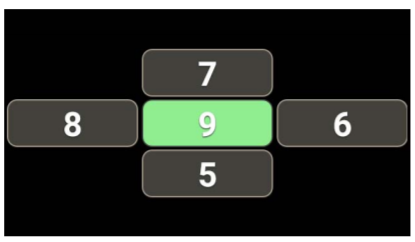
\includegraphics[scale=1.1]{gRotator.PNG}
            \caption{Demonstration of gRotator}
    \end{center}
\end{figure}
\begin{figure}[H]
    \begin{center}
        \label{abc}
            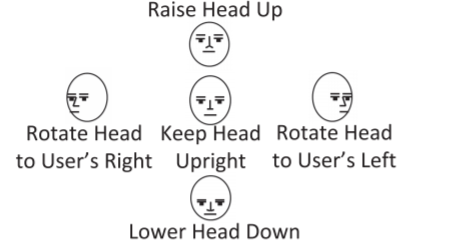
\includegraphics[scale=1.1]{headmove.png}
            \caption{Head movements in gRotator}
    \end{center}
\end{figure}
\begin{figure}[H]
    \begin{center}
        \label{abc}
            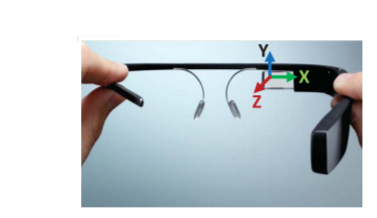
\includegraphics[scale=1.1]{motion.png}
            \caption{ A typical motion sensor coordinate system on smart glasses}
    \end{center}
\end{figure}
With the estimation of
head rotations, users can easily input password elements by
performing corresponding head rotations. Figure 4 depicts the
typical motion sensor coordinate system on the NED screen.
Generally, axis X is horizontal that points to the right; axis
Y is vertical that points to the up; and axis Z points toward
a user’s face. In terms of the angular speed, we can estimate
users’ head rotation using a dead-reckoning algorithm [17]. Let
$R_{t_{i}}$ = ($r_x$,$t_i$,$r_y$,$t_i$,$r_z$,$t_i$) be the angular speed generated by the
gyroscope at time $t_i$ . The rotation angle along each axis can be
calculated by the trapezoidal rule for integral approximation
as follows
\par  $\theta_{s,t_{i}}$ = ($r_{s,t_{i-1}}$ + $r_{s,t_{i}}$) · ($t_i$ - $t_{i-1}$)/2
 
where s $\epsilon$ \{x,y,z\} . Note that ($\theta_{x,t_i}$, $\theta_{y,t_i}$, $\theta_{z,t_i}$) is also called
as Cardan angles in 3D coordinate system [35]. For simplicity,
the angle $\theta_{x,t_i}$ and angle $\theta_{y,t_i}$ to determine the up/down
directions and left/right directions of head movements starting
from an initial head pose, which is defined as the user’s frontal
face head pose. This pose can be calibrated and set at the
moment when a user initially launches gRotator or when a
user taps on the touch-pad with two fingers together.
\par In practice, users may easily cause abrupt changes to affect
the estimation of head rotation directions, due to the inaccurate
control of head poses. For this issue, set a thresholds
$\zeta_v$ and $\zeta_h$ for up/down direction and left/right direction,
respectively. Thus, the estimation of head rotation direction
$H_{t_{i}}$ at time $t_i$ can be computed as below. \newline


\begin{figure}[H]
    \begin{center}
        \label{abc}
            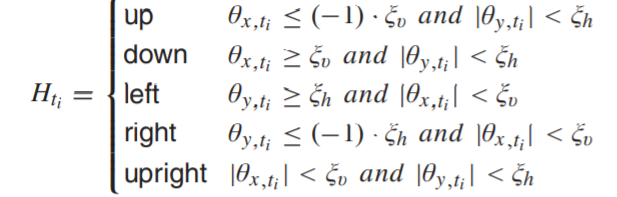
\includegraphics[scale=.5]{equation.png}
            
    \end{center}
\end{figure}


where $\zeta_v$ $\geq$ 0 and $\zeta_h$ $\geq$ 0. It is worth noting that $\theta_{x,t_i}$
and $\theta_{y,t_i}$ would be negative values if the rotation directions
of axis X and axis Y are counter-clockwise. The best performance for determining the head rotation
directions can be achieved at $\zeta_v$ = 15◦ and $\zeta_h$ = 25◦, which
is also examined in their pilot study.

\subsection{Security Analysis of gRotator}

As attackers can observe
user operations like swiping on the touch pad and head
rotations, they may know in each round whether the user
changes the number screen displayed initially and know the
exact positions of the underlying password elements located in
the displayed number screen. However, as long as the hidden
keypad, including the two number screens, is not disclosed,
the adversary would not know which number screen is chosen
by the user nor the mapping between the 5 numbers and the
positions in the displayed screen. Therefore, the adversary
cannot infer any element of the underlying password.\newline 

\textbf{Proof:} Given the user operation $op_i$ in any round i and
any two elements $p_x$ and $p_y$ in 10-sized password alphabet
\{0, 1, 2,..., 9\}, let Pr($op_i$ | $p_x$ ) and Pr($op_i$ | $p_y$ ) be the probabilities for the operation $op_i$ when the underlying password
elements are $p_x$ and $p_y$, respectively. Based on the design
of gRotator, one of the two number screens $C_s$ and $C_b$ is
randomly drawn from a uniform distribution and displayed
initially (i.e., with a probability of 1/2 ). Each number screen
contains 5 numbers whose positions are randomly shuffled.\newline
Thus we have Pr($op_i$ | $p_x$ ) = 1/2 ·Pr($p_x$ $\epsilon$ direction of $op_i$) = 1/2 · ${P_4}^4$ / ${P_5}^5$= 1/2 · ${P_4!}^5!$ = 1/10 = Pr($op_i$ | $p_y$ ) for any i, x, and
y. Thus an adversary gains no advantage for distinguishing
the i-th element in the underlying password between any
two elements in the password alphabet by observing users’
operations. \newpage


\section{gTalker}
\subsection{Design of gTalker}
The design of gTalker depends on a speech
recognition-enabled built-in microphone, which can take
a user’s speech as input. With the microphone, smart glasses
can recognize and react to the speech content. \par
For implementation, gTalker adopts the alphabet of password as $\Omega$ = {0, 1, 2,..., 9}. Figure 3.7 shows the hidden
keypad’s layout of gTalker, where every white number p is
followed by an underlined red number s. The hidden keypad
consists of two keypads, one original keypad with all white
numbers and one transformed keypad with all underlined red numbers.
\begin{figure}[H]
    \begin{center}
        \label{abc}
            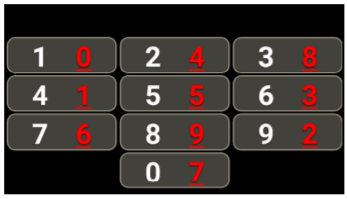
\includegraphics[scale=1.1]{gTalker.png}
            \caption{Demonstration of gTalker}
    \end{center}
\end{figure}
. In each round i, white numbers would remain their
positions while underlined red numbers would shuffle their
positions randomly. For each white number $p_k$ = k, let $s_{ik}$
denote the corresponding underlined red number in round i,
where k $\epsilon$ $\Omega$  and $s_{ik}$ $\epsilon$ $\Omega$. For 	\forall j, k $\epsilon$ $\Omega$  and j \neq k, \hspace{2}   $s_{ij}$\neq$s_{ik}$ 
holds.
\par To enter an underlying password element k, users have to
firstly identify the position of a white number $p_k$, and then
speak out the underlined red number $s_{ik}$ . For authentication,
gTalker should receive the right $p_k$ and recognize the correct
number  $s_{ik}$ said by the user. It is worth noting that the mapping
relationship between the original keypad and the transformed
keypad would not the same in each round. For example,
as shown in Figure 5, if given an underlying password element
7 and the hidden keypad, a user has to select and enter the
password element 7 and speak out 6 for authentication (note
that the white number is 7 while the followed red number is
6 in the hidden keypad).

\par To recognize a user’s input, gTalker uses an offline speech
recognition function available in Android API [18], which is
developed based on deep neural networks with hidden Markov
models (DNN-HMM) [19]. This speech recognition function is selected for gTalker, due to its speaker-independence
and low word error rate (WER) [20].

\subsection{Security Analysis of gTalker}
For gTalker, an adversary
may know the number spoken by the user in each round i.
However, as long as the transformed keypad is not disclosed, the adversary does not know the random mapping
between the original keypad and the transformed keypad.
Therefore, the adversary cannot infer the i-th element of the
underlying password in each round. \newline

\textbf{Proof:} Given the number $s_{ik}$ spoken by the user in any
round i and any two elements $p_x$ and $p_y$ in a w-sized password
alphabet (w = 10 in this implementation), let Pr(sik |px ) Pr($s_{ik}$ | $p_x$ ) and
Pr($s_{ik}$ | $p_y$ ) denote the probabilities of observing a number
$s_{ik}$ when the underlying password elements are $p_x$ and $p_y$,
respectively. Because the original keypad remains unchanged
while the transformed keypad randomly shuffles in each round,
\newline we have Pr($s_{ik}$ | $p_x$ ) = ${P_{w-1}}^{w-1}$ / ${P_w}^w$ = (w - 1)! / w! = 1/w = Pr($s_{ik}$ | $p_y$ ) for all i, x, and y. Thus an attacker gains no
advantage for distinguishing the i-th element in the underlying
password between any two elements in the password alphabet
by observing the number spoken by the user.

\chapter{DATA COLLECTION \& EVALUATION}

This section discuss about the user data collection and based on the study, evaluation of the proposed schemes. They done an IRB[25] approved user study and this section about that user study and it's results analysis.
\section{Data Collection and Methodology}
There was 57 students participated in that data collection.  It is worth noting that a
numerical identifier is assigned to each participant to protect
their privacy. In the study, each participant has to spend around
60 minutes in a quiet room and is paid with 10 dollars as compensation. In particular, the study contains three major parts,
which are developed based on a within-subjects design [40].
After completing each part, participants can have a short break
for 1-3 minutes before they move to the next part. Prior
to the main user study, they conducted a pilot study among
10 internal users in order to validate the design of the user
study procedures and select proper experimental settings and
parameters. The details of each part in the main user study are
described as below.
\begin{itemize}
    \item  The first part briefly explain the purpose of the
study to each participant, and introduce how to use
the designed schemes, including gTapper, gRotator, and
gTalker on Google Glass. More specifically, they provided
each participant with Google Glass and teach them how
to use in an interactive step-by-step manner to make sure
that every participant understands how to perform the
experiments.
\item In the second part, each participant is requested to use
gTapper, gRotator, and gTalker as three test groups.
To avoid the learning effect on the scheme performance,
all schemes are assigned to each participant in a random
sequence. In each test group, participants have to remember a password randomly generated at the beginning
and the same password would be used in the same
test group. The password is a 6-digit PIN, which has
been commonly employed in most real-world scenarios,
e.g., online banking services. If a participant forgets the
assigned password, they can use a ‘show the password’
function by swiping up with one finger on the touch pad.
\item In the last part, each participant is asked to give feedback via an online questionnaire with a 5-point Likert
scale. The online questionnaire contains 15 questions
and collects users’ knowledge background and previous
experience of smart devices, perception of the security of
user authentication, and perception and attitudes towards
the designed password entry schemes.

\end{itemize}
More specifically, in each test group, they adopted six test
conditions to evaluate the impact of time pressure and distraction during the password entry. These test conditions are used
to simulate a common and practical usage scenario when users
input their passwords. In practice, users may need to log into
a system/service emergently and complete the password entry
process within a time limit (time pressure-related conditions),
or users are interrupted and respond to tasks in emergency or
higher priority during the password entry (distraction-related
conditions). For example, a user may suspend the password
entry and rotate his/her head to talk to his/her colleague when
it is necessary. The detailed test conditions are discussed next.



\section{Test Conditions}
To simulate a practical scenario, they employed a timer
and some secondary tasks in particular tests. The timer is designed to give participants time pressure by showing how
much time left for the existing test. In a test, the timer was
implemented with a text field and displayed a countdown
number in second, at the top left corner on the NED screen.
The secondary tasks aim to simulate conditions related to
unexpected distraction. In the study, they adopted multiple
modality presented secondary tasks, which are often used in
research fields, e.g., experimental psychology [41], [42]. The
goal of using multiple modality presented secondary tasks is
to investigate the influence of modality switch in dual-task
experiments [41].
\par With these secondary tasks, the primary task can be evaluated based on the presence of different modality presentation
in the secondary tasks. The important modalities include a
linguistic modality and a spatial modality, which conduct
linguistic/spatial processes [41], [42].These two
modalities are chooses in secondary tasks, because they are common
in real-world scenarios, such as immediately responding to
chatting requests from others during the password entry. In their
tests, a participant is either required to speak out a displayed
number in a secondary task with the linguistic modality,
or required to rotate his/her head according to a displayed
direction in a secondary task with the spatial modality.
In the study, they considered the following two conditions to
test the impact of time pressure: normal condition and timed
condition.
\begin{itemize}
    \item \textbf{Normal Condition:} participants are required to minimize
their failure rate in a fixed number of login attempts without enforced time limitation. By considering a common
scenario, set the number of login attempts as 3.
\item \textbf{Timed Condition:} participants are required to reach as
many successful logins as possible within a fixed time
period. In the tests, by considering the usability, set
the time limit for gTapper and gRotator as one minute
but increase the time limit for gTalker to two minutes.
The time limits are carefully selected based on the users’
feedback and data quality requirements in their pilot study
in order to avoid the users’ uncomfortable experiences
and insufficient data in the experiments.

\end{itemize}
For secondary tasks, they defined the following distraction
levels that were used in the distraction-related test conditions.

\begin{itemize}
    \item \textbf{No Distraction :} participants only need to perform the
login task.
    \item \textbf{Distraction: } when a participant performs the login task,
a secondary task may appear with a 1/3 probability each
time asking the participant to complete a single element
entry. In particular, either a speaking number task or a
head rotation task would be selected as the secondary task
with a 1/2 probability. This aims to simulate a practical
unexpected distraction during the password entry.
    \item \textbf{Heavy Distraction :} when a participant performs the login
task, a secondary task would appear each time asking the
participant to finish a single element entry. Similar to the
above Distraction condition, either a speaking number
task or a head rotation task would be selected as the
secondary task with a 1/2 probability.
\end{itemize}
To summarize, we have 6 test conditions in each test group
through combining both time conditions and distraction levels:
normal condition with no distraction, normal condition with
distraction, normal condition with heavy distraction, timed
condition with no distraction, timed condition with distraction,
and timed condition with heavy distraction. For simplicity,
in the rest of this paper, we denote the normal condition
with no distraction and the timed condition with no distraction as normal condition and timed condition, respectively.
Further, to minimize the learning effect, each test group
would encounter these tests randomly.

\section{Experimental Results}

In this work, there are two important metrics to evaluate
the scheme performance: average login time and login success
rate. The former is used to evaluate the speed of a login
process while the latter is used to evaluate the accuracy of
login attempts. They further apply statistical analysis to measure
the significance of the experimental results. In particular,
They run an omnibus test [22] across the test conditions for
each designed scheme, and used Kruskal-Wallis test [21] to
investigate the significant differences as compared to other test
conditions.
\par 
1) Learning Curve: In the proposed schemes, it is simple and
intuitive operations to reduce the difficulty level of learning. To evaluate the performance, Figure 6 compares the
participants’ performance under the normal condition where
the 6 tests may appear at different positions in each test
group. It is found that participants spent more login time
for the tests appearing at the first position than the other
positions; however, the results are not significantly different,
i.e., it is 2.2 seconds, 1.1 seconds, and 1 second for gTapper,gRotator, and gTalker, respectively. In addition, it is found
that changing the test positions would not significantly affect
the login success rates among different schemes, in which
the rate ranged mainly between 93.1\% and 100\%. On the
whole, the results are not significantly changed with different
test positions. There are two possible reasons: 1) The training
processes are effective by providing each participant with a
detailed tutorial in an interactive step-by-step manner; and
2) THe designed schemes are easy to learn due to their simple
and intuitive operations.

\begin{figure}[H]
    \begin{center}
        \label{abc}
            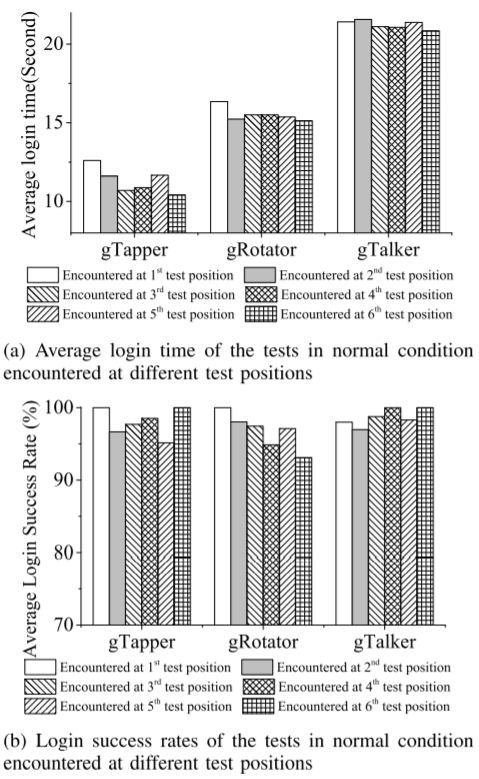
\includegraphics[scale=.8]{test1.png}
            \caption{ Learning curves for gTapper, gRotator, and gTalker.}
    \end{center}
\end{figure}

\par
2) Performance Under Normal Condition: As participants
only need to complete the login tasks without any time
pressure or secondary tasks, they use the test results under
normal condition as the baseline in their experiments.
Figure 4.1(a) shows the average time for a successful login
under normal condition for each scheme. It is seen that the
average login time for gTapper is 11.2 seconds, which was
generally shorter than the other two schemes with 15.6 seconds and 21.8 seconds for gRotator and gTalker, respectively.
To investigate the differences in login time, Figure 4.1(b) shows
the distribution of single element entry time for each scheme.
Similarly, gTapper only required 1.63 seconds regarding the
single element entry, which is much shorter than gRotator and
gTalker each with 2.20 seconds and 3.05 seconds. Regarding
the login success rate, gTapper, gRotator, and gTalker can
reach a rate of 98.3\%, 98.2\%, and 98.2\% under the normal
condition, respectively. These results indicate that participants
can make a tap task shorter than rotating head or speaking a
number on Google Glass.


\begin{figure}[H]
    \begin{center}
        \label{abc}
            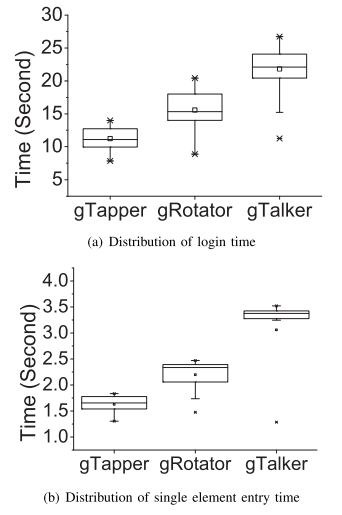
\includegraphics[scale=1.1]{avglogin.png}
            \caption{ Average login time and single element entry time.}
    \end{center}
\end{figure}
\begin{figure}[H]
    \begin{center}
        \label{abc}
            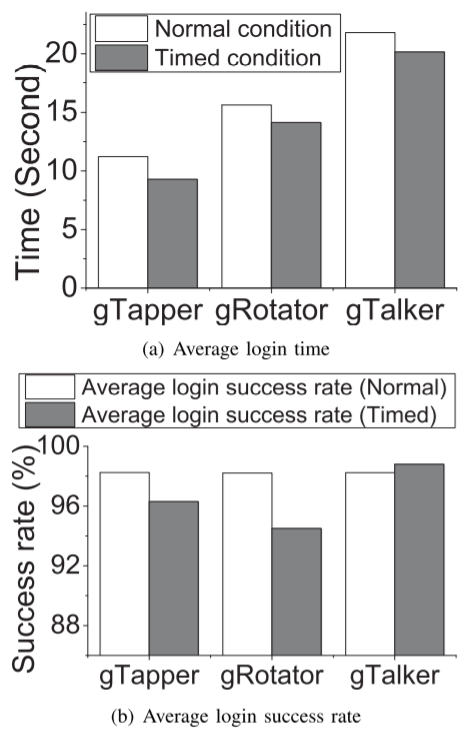
\includegraphics[scale=.8]{test2.png}
            \caption{ Impact of time pressure.}
    \end{center}
\end{figure}

\par
3) Impact of Time Pressure: Figure 8 presents participants’ performance under time pressure without distractions.
Generally, participants were found to enter passwords faster under time pressure that under normal condition, i.e., the
average time for a successful login under timed condition for
gTapper, gRotator and gTalker is 9.3 seconds, 14.1 seconds and
20.1 seconds. Similarly, participants can reduce the average
time for a single element entry, i.e., 1.36 seconds for gTapper,
1.98 seconds for gRotator, and 2.84 seconds for gTalker as
shown in Figure 9. Based on the statistical tests, they found
that there is a significant difference in login time, where
p \textless 0.001 for gTapper and p = 0.024 for gTalker (details can
refer to Table I, Table II, and Table III). These
results indicate that participants spend significantly less login time under the timed condition as compared to the normal
condition.
\begin{figure}[H]
    \begin{center}
        \label{abc}
            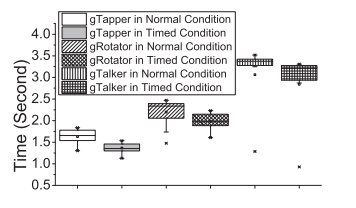
\includegraphics[scale=1.1]{avglogin2.png}
            \caption{ Distribution of single element entry time under time pressure.}
    \end{center}
\end{figure}

\begin{figure}[H]
    \begin{center}
        \label{abc}
            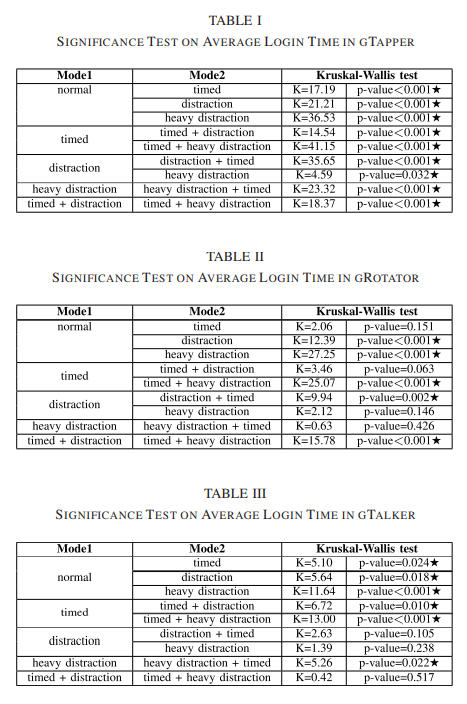
\includegraphics[scale=1]{table.png}
    \end{center}
\end{figure}

\par Regarding the average login success rates, Figure 4.3(b)
shows that participants under timed condition can achieve
96.3\% and 94.5\% for gTapper and gRotator, respectively,
which are slightly lower than the normal condition. By contrast, participants achieve a rate of 98.8\% for gTalker under
timed condition, but it is very close to that in a normal
condition. In addition, the statistical tests indicate that the
results on login accuracy under timed condition and normal
condition are not significant, i.e., the participants can still
achieve high login accuracy even under the timed condition.
This is because these tests may not be sufficiently difficult
to distinguish the impacts of test conditions due to ceiling
effect [23].So  that the results on login
accuracy are not significantly different under timed condition
as compared to normal condition.
\par
4) Impact of Distractions: Figure 4.5 shows the impact of
distractions for average time login and average login success
rate. It is observed that by raising the distraction level from
no distraction to heavy distraction, participants should spend
longer time on the login process, as well as the average time
of single element entry. The statistical results on the impact
of distractions can refer to Table I, II, and III for all three
schemes (i.e., p \textless 0.001 for gTapper in both distraction level
and heavy distraction level, p \textless 0.001 for gTapper in both
distraction level and heavy distraction level, p \textless 0.001 for
gRotator in both distraction level and heavy distraction level,
and p = 0.018 and p \textless 0.001 for gTapper in distraction level
and heavy distraction level, respectively).Therefore the login time to be significantly longer with
distraction as compared to a normal condition.
\par 
Figure 4.5(b) then shows that the average login success rates
for gTapper, gRotator and gTalker were ranged between 97.6\%
and 98.8\%, between 95.1\% and 98.2\%, and between 97\% and
98.2\%. The statistical results also indicate no significant difference in the average login success rates at different distraction
levels for all the three test groups; that is, participants can
achieve high login accuracy even with distractions. It is found that participants can reach good login
accuracy even if under distraction or heavy distraction as
compared to a normal condition.

\begin{figure}[H]
    \begin{center}
        \label{abc}
            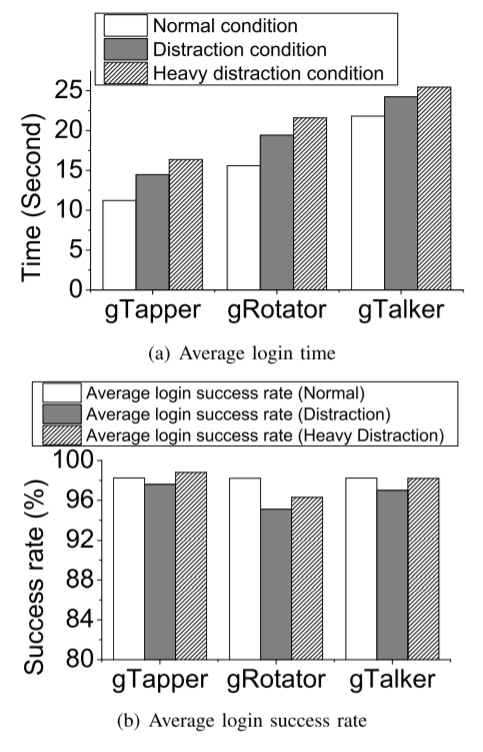
\includegraphics[scale=.8]{test3.png}
            \caption{ Impact of distraction.}
    \end{center}
\end{figure}

\begin{figure}[H]
    \begin{center}
        \label{abc}
            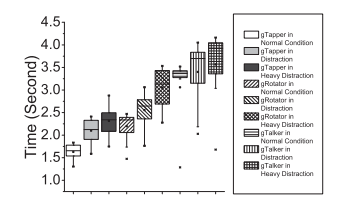
\includegraphics[scale=1.2]{avglogin3.png}
            \caption{ Distribution of single element entry time under distraction.}
    \end{center}
\end{figure}

\begin{figure}[H]
    \begin{center}
        \label{abc}
            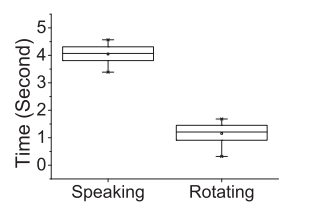
\includegraphics[scale=1.2]{second.png}
            \caption{  Distribution of time for the secondary tasks.}
    \end{center}
\end{figure}


Figure 4.7 presents the time distribution participants spent
on secondary tasks. It is observed that participants have to
take longer time for speaking number tasks than rotating head
tasks, i.e., the average time of speaking numbers and rotating
head is 4.6 seconds and 0.7 second, respectively. However,
participants can achieve an average success rate of 92\% and
100\% for speaking number tasks and rotating head tasks,
respectively. These results show that the secondary tasks could
work effectively to distract participants during the password
entry.
\par
5) Impact of Combined Conditions: They examine the
scheme performance under the combined conditions, which
can involve both time pressure and distractions simultaneously.
Compared to the tests without time pressure, the average login
time under combined conditions decreases by 2.7 seconds
on average. Their statistical results show that the difference
in the average login time is significant in most cases (i.e.,
p \textless 0.001 for gTapper in both distraction level and heavy
distraction level, p = 0.002 for gRotator in distraction level,
and p = 0.022 for gTalker in heavy distraction level).
However, the difference in the average login success rates is not significant.
 Therefore the login time is significantly shorter under timed condition
with (heavy) distraction and The login accuracy is not significantly lower under timed
condition with (heavy) distraction compared to normal condition with (heavy) distraction. It is worth noting that the time
pressure can speed up the password entry process without
greatly affect the login accuracy.
\begin{figure}[H]
    \begin{center}
        \label{abc}
            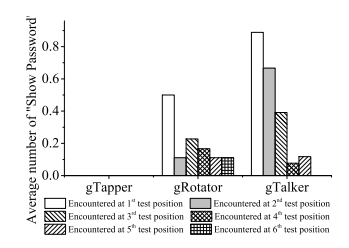
\includegraphics[scale=1]{show.png}
            \caption{Average number of “Show Password” used during the tests in normal condition encountered at different test positions}
    \end{center}
\end{figure}
6) Memory Interference: As mentioned earlier, They generated
a random password for each participant to test each scheme.
All participants are allowed to use a “Show Password” function by swiping up with one finger on the touch-pad, if they
for
get the assigned passwords. Figure 4.8 shows the average
number of “Show Password” triggered by the participants
under normal condition. Note that each test requires a participant to complete three login attempts. Their experimental
results show that no “Show Password” was used by the
participants during the test of gTapper. For gRotator and
gTalker, participants used the “Show Password” more often in
the tests appearing at first position than other positions. This is
because participants may gradually get more familiar with the
assigned password. For the tests appearing at the last position,
the average number of using “Show Password” decreases to
only 0.1 times for gRotator and 0 times for gTalker. The results
indicate that the schemes do not incur significant interference
on password recall.
\par 
7) Users’ Perception: In this study, They collect users’ perception and feedback through online questionnaires. As shown
in Figure 4.9, most participants found that the proposed  schemes are
easy to learn and could be more secure than the existing
password entry methods used on Google Glass. In particular,
gTapper is the most popular among the three schemes, i.e., all
of the participants are willing to use gTapper, while 56.1\% and
58.5\% of participants are willing to use gRotator and gTalker,
respectively. \newline 
\par 
8) Comparison With Existing Password Entry Method on
Smart Glasses in Practice: In this part,  compare proposed
password entry schemes with the existing real-world password
entry methods available on commodity smart glasses, such
as Google Glass and HoloLens. Most current password entry
methods require users to input their passwords in plaintext via a standard keyboard on PCs or a touch screen on
mobile phones, which are connected to their smart glasses. It is worth emphasizing that the proposed
schemes aim to preserve the benefits of traditional password
entry schemes on smart glasses, and further improve their
security and practicability.

\begin{figure}[H]
    \begin{center}
        \label{abc}
            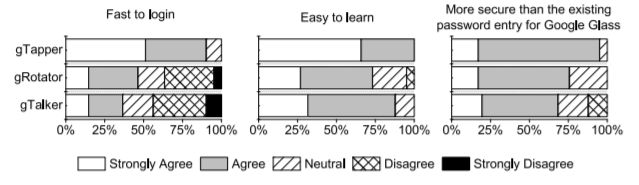
\includegraphics[scale=1]{comp1.png}
            \caption{Perception of participants.}
    \end{center}
\end{figure}


Table IV shows a scheme comparison based on
the security-deployability-usability metrics. In particular, the metrics related
to security focus on anti-eavesdropping of password,
which correspond to the rows from “Resilient-to-PhysicalObservation” to “Unlinkable”. The metrics of deployability
highlight the practicability of password entry schemes,
which correspond to the rows from “Accessible” to “NonProprietary”. The metrics of usability pay attention to
the usability costs, which correspond to the rows from
“Nothing-to-Carry” to “Easy-Recovery-from-Loss”.

\par
The comparison indicates that the designed schemes are
able to improve the security level by offering the benefits of Resilient-to-Physical-Observation, No-Trusted-ThirdParty and partial benefit of Resilient-to-Internal-Observation,
because the proposed schemes are secure against external eavesdropping attacks and unprivileged internal eavesdropping attacks
without relying on any trusted third party. For deployability,
the proposed  schemes can provide the benefit of Negligible-Cost-perUser, as they use common built-in hardware on smart glasses
only, whereas the other methods need additional PCs or
mobile phones to connect with smart glasses. For usability, the
schemes can preserve most benefits of existing entry methods,
and provide the benefit of Nothing-to-Carry, which is only
partially offered by most other methods.

\begin{figure}[H]
    \begin{center}
        \label{abc}
            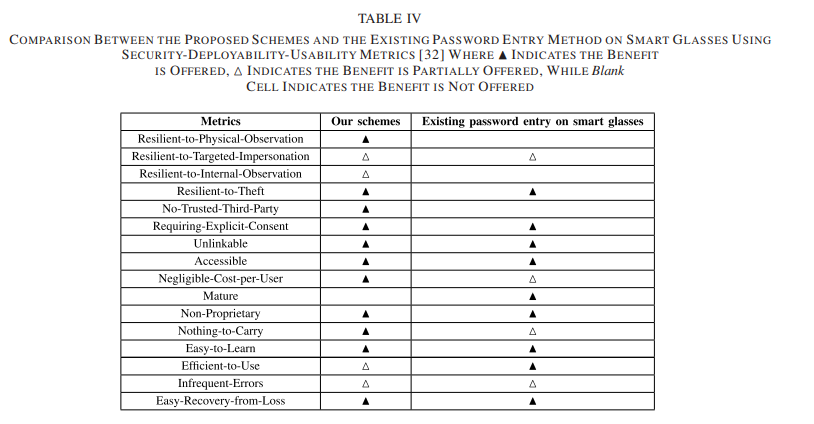
\includegraphics[scale=1]{table2.png}
    \end{center}
\end{figure}



\chapter{DISCUSSION}

\section{Security and Usability by Extending Password
Alphabet and Length}
The current schemes adopt a 6-digit password, while we
can raise the security level of the schemes by using a longer
password and a richer password for certain scenarios with
higher security requirements, such as online banking.
\par On one hand, applying a longer password is a direct way
to raise the security level as additional rounds of password
element entry associated with more hidden random keypads
are involved. However, simply enlarging password length may introduce higher time cost of user
authentication process and more memory efforts by users,
which could eventually affect the usability of the schemes.
\par 
On the other hand, it is not difficult to achieve higher security level by enlarging a password space with a richer password
alphabet . For a richer password alphabet, proposed schemes
can be easily adjusted. For example, by given a password
alphabet with 36 elements, including digits 0 to 9 and letters
a to z, gTapper’s screen can be adjusted to accommodate
36 grids for the password alphabet. By displaying more grids,
it is necessary to accelerate focus cursor moving by allowing
long-distance shifts. For gRotator, we can modify the screen
layout to 18 elements, so that a user may select an element by
rotating his/her head to a correct position among 18 positions.
For gTalker, both original keypad and transformed keypad
can be adjusted to include all 36 elements in the password
alphabet. To enter an element on the original keypad, a user has
to speak out the corresponding letter or digital number on the
transformed keypad (see the implementation details of gTalker
in Section IV-E). The richer password alphabet could introduce
more elements to be displayed and chosen by users and result
in usability cost during user operations, but the usability of proposed 
schemes can be further mitigated and optimized by making
clever tradeoffs between password alphabet and password
strength, i.e., a richer password alphabet only requires a shorter
password length to achieve the same password strength. Due
to the complexity, it is leave it as one of the further directions.



\section{Advantages}

The main advantages of the proposed system are: \begin{itemize}
    \item The proposed scheme has a better way of authentication when compared to the existing schemes. As different methods are used in the proposed scheme  the eavesdropping attackers cannot be able to track any clue about the password elements. Therefore we can say that the proposed system is more secure than conventional password entry within the limited hardware.
    \item The designed
schemes do not need any additional hardware other than
a touch pad, a gyroscope, and a microphone, which
are commonly available on smart glasses. In this case,
proposed schemes have a big potential to be implemented on
commodity smart glasses in practice.
\item As the google glass has a compact size and the proposed scheme doesn't use any additional hardware like keyboard, mouse, mobile, laptop etc., the users can easily enter there password even in the outdoors because of the NED screen and the better entry schemes in the proposed system.
\item The proposed schemes doesn't use any external hardware. The schemes uses Touch pad, Gyroscope and Microphone which is already available in the google glasses.
\end{itemize}

\section{Limitations}


\begin{itemize}
    \item \textbf{Ecological validity:}This is an open challenge to most
research in this area. The participants were
mainly from universities who may be usually more active to
use smart wearable products such as smart glasses. There is
always a need to consider other population and include even
larger sample size.
    \item \textbf{Password alphabet:} . How to include full password alphabet
is a challenge, including digits, case sensitive letters and
symbols. Due to the compact design of NED screen on smart
glasses, it is very difficult to display too many characters on
such small screen at the same time. One potential solution
is to use multiple screens; however, users may need to frequently change among multiple screens in order to identify
their password elements. This may harm the usability of the
password entry schemes. Fortunately, emerging techniques like
augmented reality and virtual reality could allow users to access on screens with wider views and more user-friendly
interactions. For example, eye-gaze based interaction may be
available for users to input passwords on future smart glasses,
based on the eye gaze and movements. With the eye-gaze
based interaction, a user may quickly identify and select target
elements on the NED screen.

\item \textbf{Speech recognition:} This is a necessary functionality for
gTalker, and its performance is mainly decided by the accuracy
and the time consumption for recognizing a number said by
a user. This is similar to most systems that employ speech
recognition [18]. Compared to traditional typing based input,
speech recognition-based input does not have any advantages
in accuracy or speed if the input is not a sentence but a
single character like password element. This is because
saying a word is usually slower than a single tap. As the
implementation adopts a general speech recognition function
provided by Google’s Android API, the input of proposed schemes
only involves 10 single-digit numbers. To solve this issue, the
implementation includes all homophones for the 10 singledigit numbers, and can improve the recognition rate to 93\%
in the study. In future, it is an interesting topic to investigate
how to train a speech recognition model to achieve even higher
accuracy and shorter login time.

\item \textbf{Head movement estimation:} How to accurately estimate
head movements in gRotator using inertial sensors is still
a challenge on smart glasses. The main factors include the
cumulative errors of dead-reckoning based estimation algorithms and the accuracy of inertial sensors. All dead-reckoning
based algorithms are subject to cumulative errors, because
they estimate a current position based on a pre-determined
position. The accuracy of inertial sensors on existing
smart glasses is still not high. Fortunately, the accuracy of
inertial sensors would improve fast with better hardware. This
trend will lead to better performance of gRotator.
\end{itemize}

\section{Overview of scheme analysis}
By summing up the entire results, we can take a look at some of the major points in this section.
\begin{itemize}
    \item The results indicate that participants spend significantly less login time under the timed condition as compared to the normal
condition.
    \item  The results on login
accuracy are not significantly different under timed condition
as compared to normal condition.
\item  The login time to be significantly longer with
distraction as compared to a normal condition.
\item Participants can reach good login
accuracy even if under distraction or heavy distraction as
compared to a normal condition.
\item The login time is significantly shorter under timed condition
with (heavy) distraction.
\item t the login accuracy is not significantly lower under timed
condition with (heavy) distraction compared to normal condition with (heavy) distraction. It is worth noting that the time
pressure can speed up the password entry process without
greatly affect the login accuracy.


\end{itemize}





\chapter{CONCLUSION AND FUTURE ENHANCEMENT}

At present, most existing anti-eavesdropping password entry
schemes on smart glasses are heavily depending on additional
PCs or mobile devices connected to smart glasses, while the
required devices may not be always available in a real scenario,
e.g., public areas and outdoors. This requires users to switch
between different systems and devices, which may cause interrupted experience and significantly degrade the practicability
and usability of smart glasses. This paper focus on
this challenge and propose three anti-eavesdropping password
entry schemes for smart glasses: named gTapper, gRotator
and gTalker. These schemes can protect the password entry
by breaking the correlation between the underlying password
and the interaction observable to adversaries. In addition, the proposed
schemes do not need extra hardware beyond what is commonly
available on existing smart glasses. Based on the analysis of  IRB-approved users study with
57 participants conducted by them, and found that the designed schemes are easy
to use in various real-world scenarios. \newline 
\par As a future scope, we can improve the proposed scheme by using vast possibilities of Augmented Reality and Virtual Reality[15].
In the proposed schemes, there is a limitation in the size of NED screen display and so that the password length is very less. In this era, we need more complex passwords which require more alphabet sets. But we cannot include every keys in keyboard in the NED screen as it is very small. So that we need to implement this using AR-VR to rich the set of alphabet.
\begin{figure}[H]
    \begin{center}
        \label{abc}
            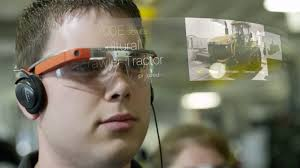
\includegraphics[scale=1]{ar.jpg}
            \caption{Demonstration of AR-VR in Google glasses.}
    \end{center}
\end{figure}
\par In the nearly future, the smart glasses will be have more hardware as in mobile phones, tablets etc.
When there will be a biometrics[24] hardware available in the google glasses, there is a scope of Bio-metric sensors like fingerprint recognition, iris
recognition etc. for password entry.

\begin{figure}[H]
    \begin{center}
        \label{abc}
            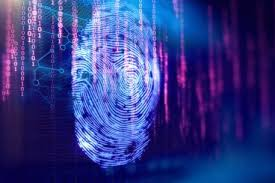
\includegraphics[scale=1]{bio.jpeg}
            \caption{Biometrics.}
    \end{center}
\end{figure}

  

%\chapter{REFERENCES}
\renewcommand{\bibname}{\uppercase{REFERENCES}}
\begin{thebibliography}{999}
\addcontentsline{toc}{chapter}{\hspace{0.19in} REFERENCES}

\bibitem{a}{ Yan Li, Y. Cheng,Weizhi Meng, Yingjiu Li and R. H. Deng \textquotedblleft Designing Leakage-Resilient Password Entry on
Head-Mounted Smart Wearable Glass Devices", \textit{ IEEE TRANSACTIONS ON INFORMATION FORENSICS AND SECURITY}, Volume: 16, Issue: 5, July 2020.  }

\bibitem{b}{Y. Li, Y. Cheng, Y. Li, and R. H. Deng \textquotedblleft What you see is not
what you get: Leakage-resilient password entry schemes for smart
glasses,” \textit{ Computer Community}, in Proc. ACM Asia Conf. Comput. Commun. Secur., April 2017,
pp. 327–333  }

\bibitem{c} 	 {{\textquotedblleft Google. (2017). Google Glass\textquotedblright}. [Online]. Available:\\ \textit{https://developers.google.com/glass/distribute/glass-at-work} Accessed on: Sept. 28, 2020}

\bibitem{d} {\textquotedblleft  Microsoft. (2017). Microsoft Hololens \textquotedblright . [Online]. Available:\\ \textit{https://www.microsoft.com/microsoft-hololens/en-us} Accessed on: Sept. 28, 2020}


\bibitem{e}{Q. Yan, J. Han, Y. Li, J. Zhou, and R. H. Deng \textquotedblleft Designing leakage resilient password entry on touchscreen mobile devices,” \textit{ Computer Community}, in Proc. 8th ACM SIGSAC Symp. Inf., Comput. Commun. Secur., 2013, pp. 37–48  }

\bibitem{f}{P. D. Adamczyk and B. P. Bailey \textquotedblleft If not now, when?: The effects of interruption at different moments within task execution,” \textit{ NDSS}, in Proc. Conf. Hum. Factors Comput. Syst., 2004, pp. 271–278}

\bibitem{g} 	 {{\textquotedblleft  Augmented Reality-Virtual Reality\textquotedblright}. [Online]. Available:\\ \textit{https://learningenglish.voanews.com/a/augmented-reality-versus-virtual-reality/3844772.html} Accessed on: Oct. 12, 2020}

\bibitem{h} 	 {{\textquotedblleft FOV \textquotedblright}. [Online]. Available:\\ \textit{https://en.wikipedia.org/wiki/Field_of_view} Accessed on: Oct. 12, 2020}

\bibitem{i} { L. Ginzburg, P. Sitar, and G. K. Flanagin, \textquotedblleft User authentication system
and method,”  U.S. Patent 7 725 712, April 2017, May 25, 2010,
pp. 327–333  }
\bibitem{j}{ D. Weinshall,\textquotedblleft Cognitive authentication schemes safe against spyware,”  in Proc. IEEE Symp. Secur. Privacy, 2006. p. 6  }

\bibitem{k}{ Q. Yan, J. Han, Y. Li, and R. Deng,\textquotedblleft On limitations of designing usable
leakage-resilient password systems: Attacks, principles and usability,”  in
Proc. NDSS, 2012, pp. 1–7.  }

\bibitem{l} 	 {{\textquotedblleft Eavesdropping attack \textquotedblright}. [Online]. Available:\\ \textit{https://www.sciencedirect.com/topics/computer-science/eavesdropping-attack} \newline Accessed on: Oct. 12, 2020}

\bibitem{m} 	 {{\textquotedblleft Smart Wearable Devices \textquotedblright}. [Online]. Available:\\ \textit{https://www.gadgetsnow.com/slideshows/8-smart-wearables-you-must-know-about/photolist/51256562.cms} Accessed on: Oct. 12, 2020}

\bibitem{n} 	 {{\textquotedblleft Network Traffic Monitor \textquotedblright}. [Online]. Available:\\ \textit{https://www.solarwinds.com/network-bandwidth-analyzer-pack/use-cases/network-traffic-monitor} Accessed on: Oct. 12, 2020}

\bibitem{o} 	 {{\textquotedblleft VR-AR based payment \textquotedblright}. [Online]. Available:\\ \textit{https://www.fintechmagazine.com/digital-payments/vr-ar-and-future-payments}\newline Accessed on: Oct. 12, 2020}

\bibitem{p} 	 {{\textquotedblleft Wikipedia. Gyroscope \textquotedblright}. [Online]. Available:\\ \textit{https://en.wikipedia.org/wiki/Gyroscope} Accessed on: Oct. 12, 2020}

\bibitem{q} 	 {{\textquotedblleft Wikipedia. Dead Reckoning Algorithm \textquotedblright}. [Online]. Available:\\ \textit{https://en.wikipedia.org/wiki/Dead_reckoning} Accessed on: Oct. 12, 2020}

\bibitem{r} 	 {{\textquotedblleft Android. Speech Recognition in Android API \textquotedblright}. [Online]. Available:\\ \textit{https://developer.android.com/reference/android/speech/SpeechRecognizer} Accessed on: Oct. 12, 2020}

\bibitem{s}{Longfei Li, Yong Zhao, Dongmei Jiang, Yanning Zhang, Fengna Wang, Isabel Gonzalez, Enescu Valentin, Hichem Sahlig \textquotedblleft Hybrid Deep Neural Network--Hidden Markov Model (DNN-HMM) Based Speech Emotion Recognition", \textit{ IEEEexplore Humaine Association Conference on Affective Computing and Intelligent Interaction}, 12 December 2013.  }

\bibitem{t} 	 {{\textquotedblleft Wikepedia. Word Error Rate(WoR) \textquotedblright}. [Online]. Available:\\ \textit{https://en.wikipedia.org/wiki/Word_error_rate} Accessed on: Oct. 12, 2020}

\bibitem{u} 	 {{\textquotedblleft Statisticshowto. Kruskal Wallis Test \textquotedblright}. [Online]. Available:\\ \textit{https://www.statisticshowto.com/kruskal-wallis/} Accessed on: Oct. 12, 2020}

\bibitem{v} 	 {{\textquotedblleft Wikepedia. Omnibus test \textquotedblright}. [Online]. Available:\\ \textit{https://en.wikipedia.org/wiki/Omnibus_test} Accessed on: Oct. 12, 2020}

\bibitem{w} 	 {{\textquotedblleft Wikepedia. Ceiling effect \textquotedblright}. [Online]. Available:\\ \textit{https://en.wikipedia.org/wiki/Ceiling_effect_(statistics)} Accessed on: Oct. 12, 2020}

\bibitem{x} 	 {{\textquotedblleft Wikepedia. Biometrics \textquotedblright}. [Online]. Available:\\ \textit{https://en.wikipedia.org/wiki/Biometrics} Accessed on: Oct. 12, 2020}

\bibitem{y} 	 {{\textquotedblleft Wikepedia. IRB \textquotedblright}. [Online]. Available:\\ \textit{https://en.wikipedia.org/wiki/IRB_Infrastructure} Accessed on: Oct. 12, 2020}



\end{thebibliography}

\end{document}